\chapter{Design Study - Solar Cell Experiment}\label{CH:Design1}
This subsystem design was part of the FIREBIRD-II mission, and was an electronic load used to measure the performance of a spacecraft's solar cells on orbit. By working with an industry partner, the SSEL was able to utilize cutting edge solar cell technology in exchange for providing the customer with low-cost flight heritage and useful environmental data. This chapter will focus on the design method used to fulfill the requirements as defined by the collaboration between the SSEL team and the customer. After discussing the subsystem requirements, the concept design can take shape, followed by the analyses and calculations performed to verify circuit functionality. 

At this time, the SSEL relied on the Mentor Graphics PADS Suite for electrical computer aided design (ECAD), and integrated SPICE simulation was not a feature that was readily available. Therefore, simulations of the critical circuits and subcircuits was performed using LTSpice developed by Linear Technology. Then, a full schematic was captured in PADS for creating the PCB layout files and bill-of-materials needed for fabrication and assembly of the subsystem. 

\section{Requirements and Conceptual Design}\label{Sect:test}



\begin{figure}[htbp]
	\centering
	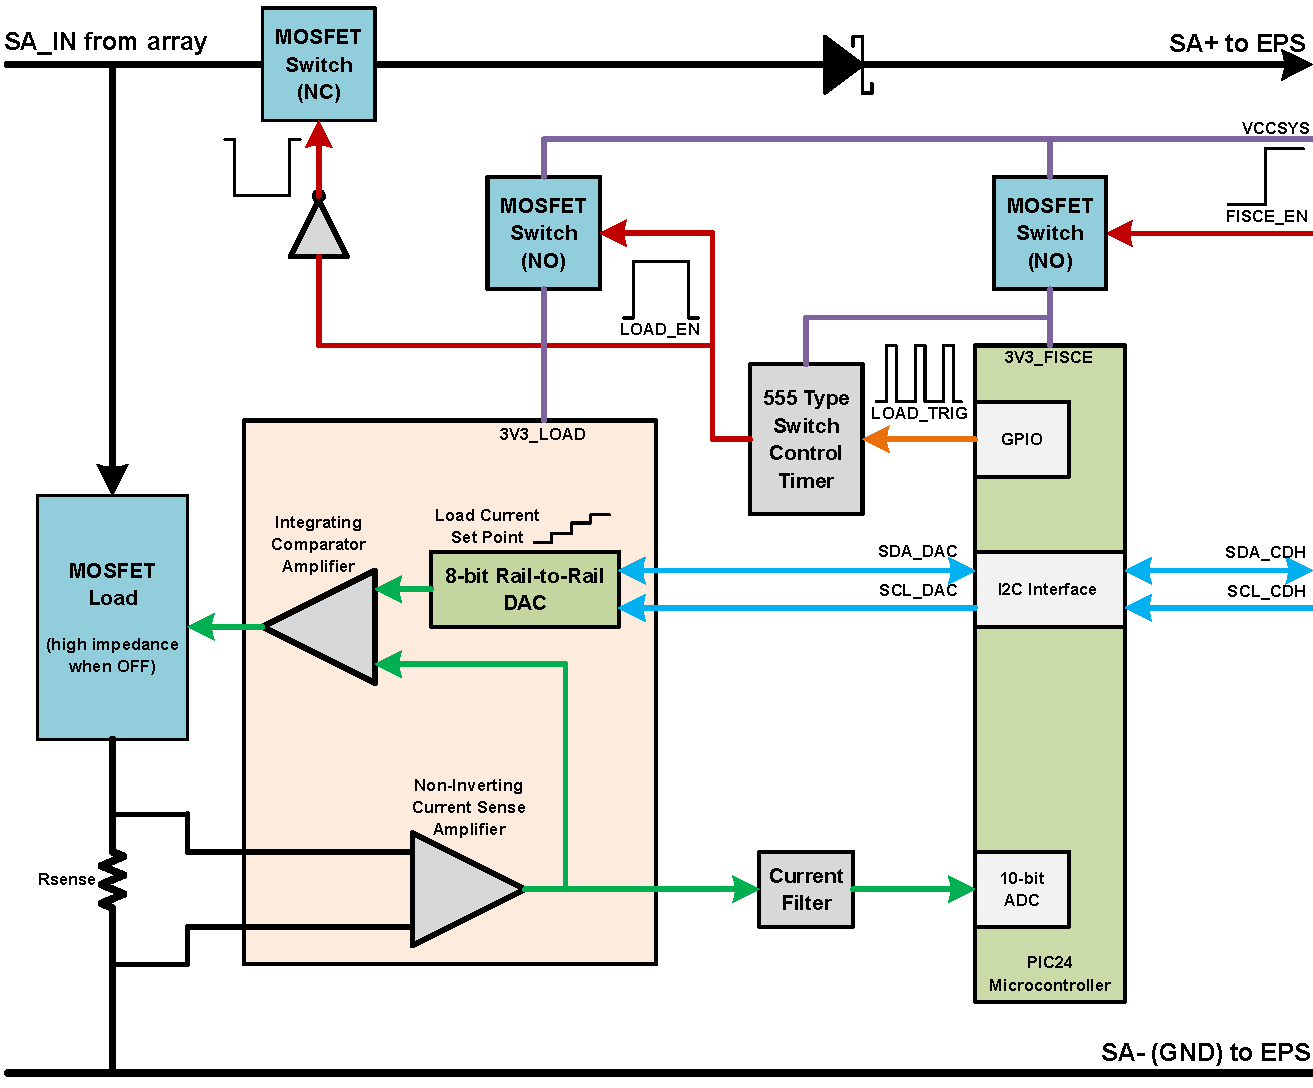
\includegraphics[width=\textwidth]{../figs/fisce/concept/fisce_panel_diagram_load_control.pdf}
	\caption{This block diagram represents the components of the FISCE load circuit and their functions.}
	\label{fig:plot}
\end{figure}



\section{Circuit Simulations and Calculations}\label{Sect:test}



\section{PCB Layout and Mechanical Design}\label{Sect:test}

\begin{figure}[htbp]
	\centering
	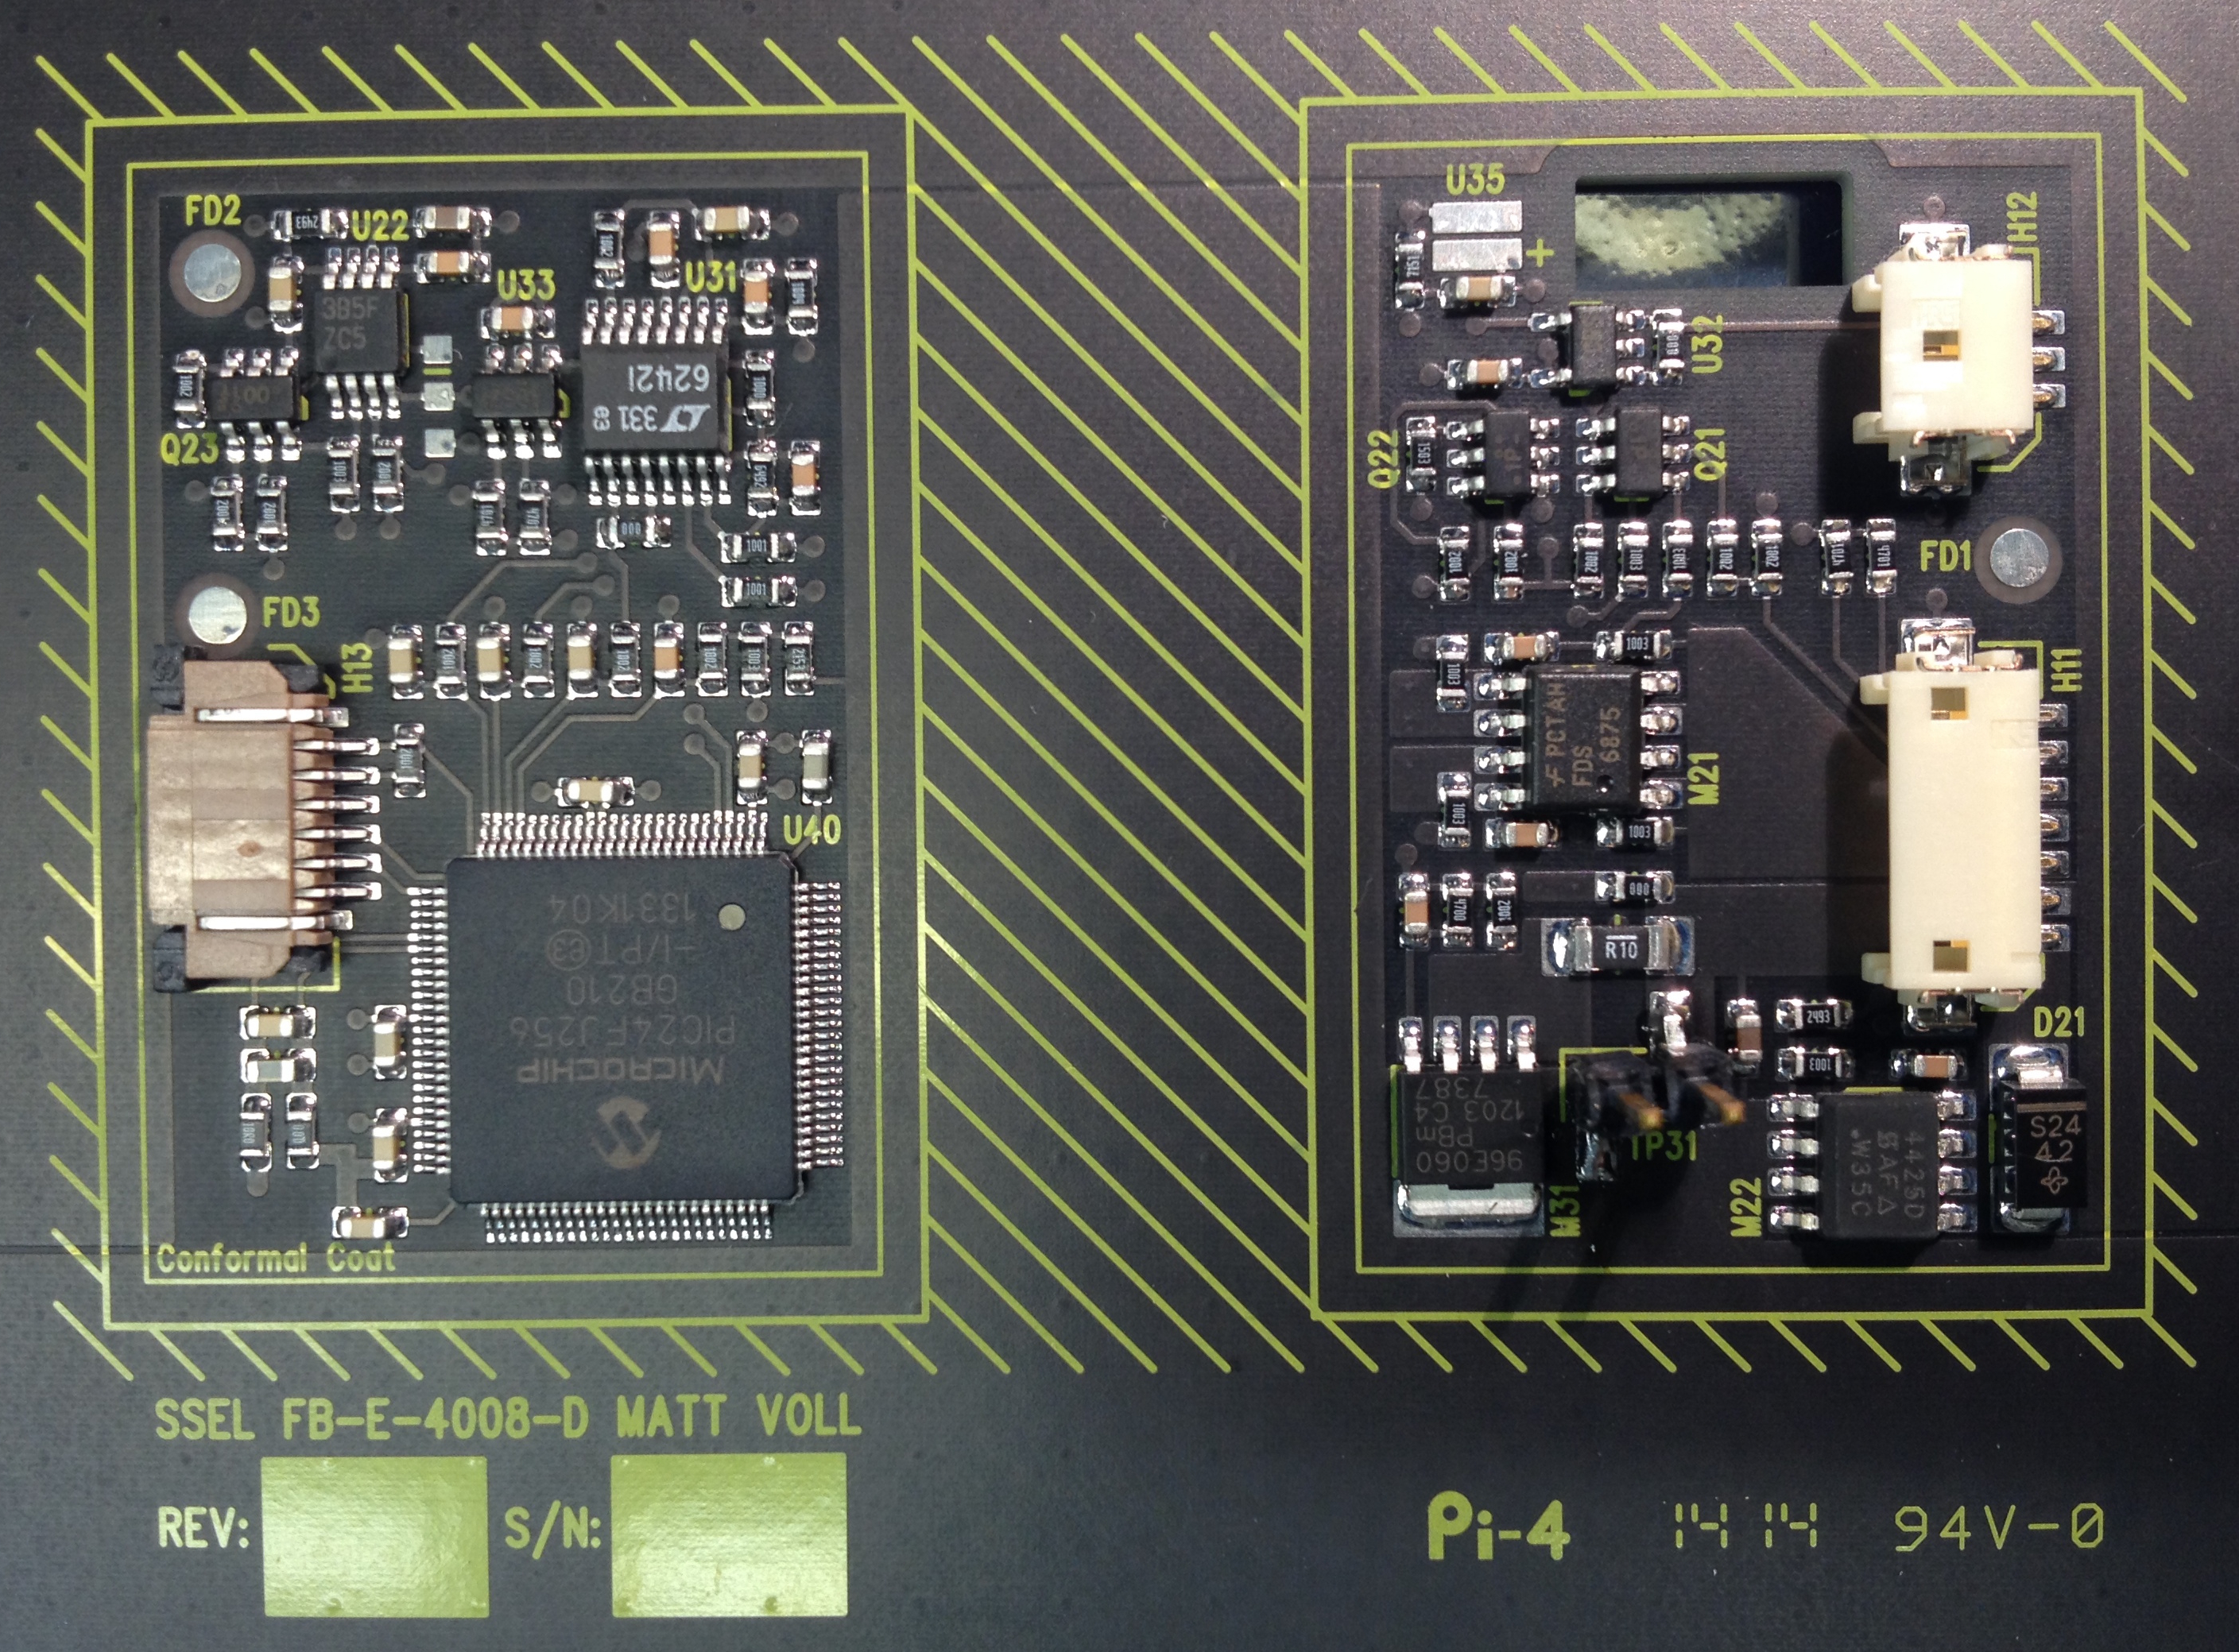
\includegraphics[width=\textwidth]{../figs/fisce/manufacturing/fisce_assembled.jpg}
	\caption{The assembled FISCE load circuit on the backside of the solar panel substrate.}
	\label{fig:photo}
\end{figure}

\section{Calibration and Results}\label{Sect:test}
